%%%%%%%%%%%%%%%%%%%%%%%%%%%%%%%%%%%%%%%%%%%%%%%%%%%%%%%%%%%%%%%%%%%
%TO AVOID FORMATTING ISSUES, COMPILE THIS ONLY AT WWW.OVERLEAF.COM%
%%%%%%%%%%%%%%%%%%%%%%%%%%%%%%%%%%%%%%%%%%%%%%%%%%%%%%%%%%%%%%%%%%%
%AUTHOR: ABHINAV BAKSHI
%CLASS:  BE C 302
%%%%%%%%%%%%%%%%%%%%%%%%%%%%%%%%%%%%%%%%%%%%%%%%%%%%%%%%%%%%%%%%%%%
\documentclass[a4paper,12pt]{article}
\usepackage{graphicx}
%To use this font, you need XeTex or LuaTex, prefer openleaf
\newenvironment{codefont}{\fontfamily{ccr}\selectfont}{\par}

\title{
	\normalfont \normalsize 
	\textsc{Pimpri Chinchwad College of Engineering \\ 
		Computer Laboratory - IV} \\
	[10pt] 
	\rule{\linewidth}{0.5pt} \\[6pt] 
	\huge Assignment No - A4 \\
	\rule{\linewidth}{2pt}  \\[10pt]
}
\author{}
\date{\normalsize}


\begin{document}
\maketitle

%%%%%%%%%%%%%%%%%%%%%%%
% FOR A NUMBERED LIST
% \begin{enumerate}
% \item Your_Item
% \end{enumerate}
%%%%%%%%%%%%%%%%%%%%%%%
% FOR A BULLETED LIST
% \begin{itemize}
% \item Your_Item
% \end{itemize}
%%%%%%%%%%%%%%%%%%%%%%%
% TO IMPORT AN IMAGE
% \includegraphics[width=\textwidth]{name_of_file}
% \textwidth makes the picture the width of the paragraphs
%%%%%%%%%%%%%%%%%%%%%%%%%%%%%%
% TO CREATE A FIGURE WITH A NUMBER AND CAPTION
% \begin{figure}
% \includegraphics[width=\textwidth]{image}
% \caption{Your Caption Goes Here}
% \label{your_label}
% \end{figure}
% REFER TO YOUR FIGURE LATER WITH
% \ref{your_label}
% LABELS NEED TO BE ONE WORD
%%%%%%%%%%%%%%%%%%%%%%%%%%%%%
% TO ADD CODE
% \begin{codefont}
% Some code in "courier" font
%\end{codefont}
%%%%%%%%%%%%%%%%%%%%%%%%%%%%%
\section{Aim}
	\paragraph{} Write a program on an unloaded cluster for several different numbers of nodes and record the time taken
	in each case. Draw a graph of execution time against the number of nodes.
	
\section{Objective}
	\begin{itemize}
		\item To understand the concept of clustering  
		\item To understand the applications of MPI  
		
	\end{itemize}
	
\section{Mathematical Model}
	Let S = \{ s, e, x, y, Fm, Si, DD, NDD, Memshared \} \\
	s = Initial State, i.e. Set of individual Nodes/Computers \\  
	e = End State, i.e. Set of Nodes working together \\	 
	Si = Intermediate state i.e. Setting up the nodes together as a cluster  \\
	x = Input values i.e. Values for a given computation problem y = Output/Result i.e. Computed Solution \\	 
	Fm = Main function or algorithm that gives specific output i.e. main () function i.e.  	Computation solution to the problem given. \\
	NDD = Non deterministic data i.e. the Values shared between Nodes for computation  	purpose. \\
	DD = Deterministic data i.e. Intermediate Values of computation between nodes.\\
	 Memshared = The Shared Memory (SM) used for Data Processing. \\
	
	
	
\section{Theory}
\subsection{Clustering:} 
\paragraph{} A computer cluster consists of a set of loosely or tightly connected computers that work together so that, in many respects, they can be viewed as a single system. Unlike grid computers, computer clusters have each node set to perform the same task, controlled and scheduled by software. 

\paragraph{} The components of a cluster are usually connected to each other through fast local area networks ("LAN"), with each node (computer used as a server) running its own instance of an operating system. In most circumstances, all of the nodes use the same hardware and the same operating system, although in some setups (i.e. using Open Source Cluster Application Resources (OSCAR)), different operating systems can be used on each computer, and/or different hardware. \\

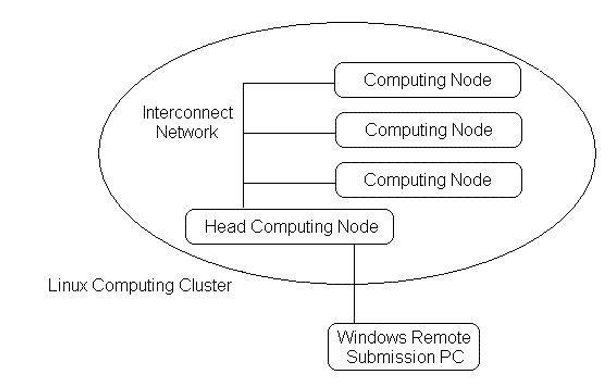
\includegraphics[width = \textwidth]{clustertime_diag}
		
\paragraph{} They are usually deployed to improve performance and availability over that of a single computer, while typically being much more cost-effective than single computers of comparable speed or availability. 

\paragraph{} Computer clusters emerged as a result of convergence of a number of computing trends including the availability of low-cost microprocessors, high speed networks, and software for high-performance distributed computing. They have a wide range of applicability and deployment, ranging from small business clusters with a handful of nodes to some of the fastest supercomputers in the world such as IBM's Sequoia. The applications that can be done however, are nonetheless limited, since the software needs to be purpose-built per task. It is hence not possible to use computer clusters for casual computing tasks. 

\paragraph{} A computer cluster may be a simple two-node system which just connects two personal computers, or may be a very fast supercomputer. A basic approach to building a cluster is that of a Beowulf cluster which may be built with a few personal computers to produce a cost-effective alternative to traditional high performance computing. An early project that showed the viability of the concept was the 133-node Stone Supercomputer. The developers used Linux, the Parallel Virtual Machine toolkit and the Message Passing Interface library to achieve high performance at a relatively low cost. 

\subsection{MPI: }
\paragraph{} MPI is a language-independent communications protocol used for programming parallel computers. Both point-to-point and collective communication are supported. MPI "is a message-passing application programmer interface, together with protocol and semantic specifications for how its features must behave in any implementation." MPI's goals are high performance, scalability, and portability. MPI remains the dominant model used in highperformance computing today. \\
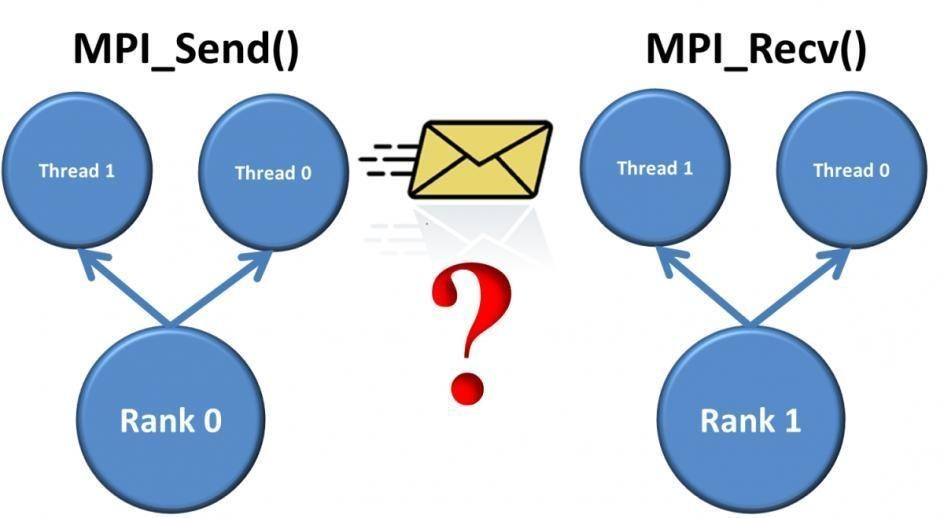
\includegraphics[width = \textwidth]{clustertime_diag2}
\paragraph{} MPI is not sanctioned by any major standards body; nevertheless, it has become a de facto standard for communication among processes that model a parallel program running on a distributed memory system. Actual distributed memory supercomputers such as computer clusters often run such programs. The principal MPI-1 model has no shared memory concept, and MPI-2 has only a limited distributed shared memory concept. Nonetheless, MPI programs are regularly run on shared memory computers. Designing programs around the MPI model (contrary to explicit shared memory models) has advantages over NUMA archi tectures since MPI encourages memory locality. 
\paragraph{} Although MPI belongs in layers 5 and higher of the OSI Reference Model, implementations may cover most layers, with sockets and Transmission Control Protocol (TCP) used in the transport layer. 
\paragraph{} Most MPI implementations consist of a specific set of routines (i.e., an API) directly callable from C, C++, Fortran and any language able to interface with such libraries, including C\#, Java or Python. The advantages of MPI over older message passing libraries are portability (because MPI has been implemented for almost every distributed memory architecture) and speed (because each implementation is in principle optimized for the hardware on which it runs). 
\paragraph{} MPI uses Language Independent Specifications (LIS) for calls and language bindings. The first MPI standard specified ANSI C and Fortran-77 bindings together with the LIS. The draft was presented at Supercomputing 1994 (November 1994) and finalized soon thereafter. About 128 functions constitute the MPI-1.3 standard which was released as the final end of the MPI-1 series in 2008. 

\section{Testing:}
\subsection{Positive Testing}
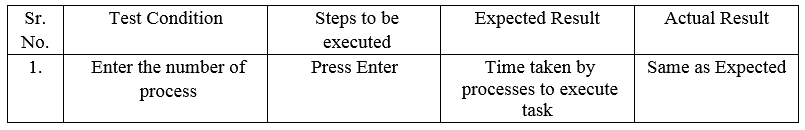
\includegraphics[width = \textwidth]{clustertime_positive}
\subsection{Negative Testing}
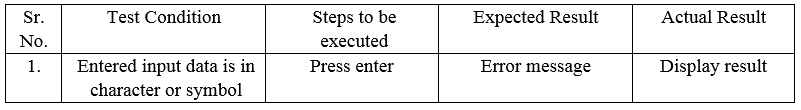
\includegraphics[width = \textwidth]{clustertime_negative}

\section{Algorithm}
\begin{enumerate}
	\item Start
    \item Assign a task to every node such that it consumes a significant amount of time
    \item Each node will complete the task and will compute the total time taken
    \item All nodes will return the total time taken to the master node
    \item The master node will read the time taken by each node and will write it to the output file
    \item A graph will be generated based on the values of output file using $QuickPlot$
    \item Stop
\end{enumerate}

\section{Conclusion}
 
 Thus we studied concept of clustering, which consists of a set of loosely or tightly connected computers that work together and created a program on an unloaded cluster for several different numbers of nodes and record the time taken in each case. 
 

\vspace{20px}
\begin{center}
	\begin{tabular}
		{|c|c|c|c|}\hline
		{\bf Roll No.}		&{\bf Name of Student}		&{\bf Date of Performance}  				&{\bf Date of Submission}  \\ \hline
		{302}	&	{Abhinav Bakshi }& {6/1/16}	&  {20/1/16}\\ \hline
	\end{tabular}\\ 
\end{center}

\section{Plagarism Report}
	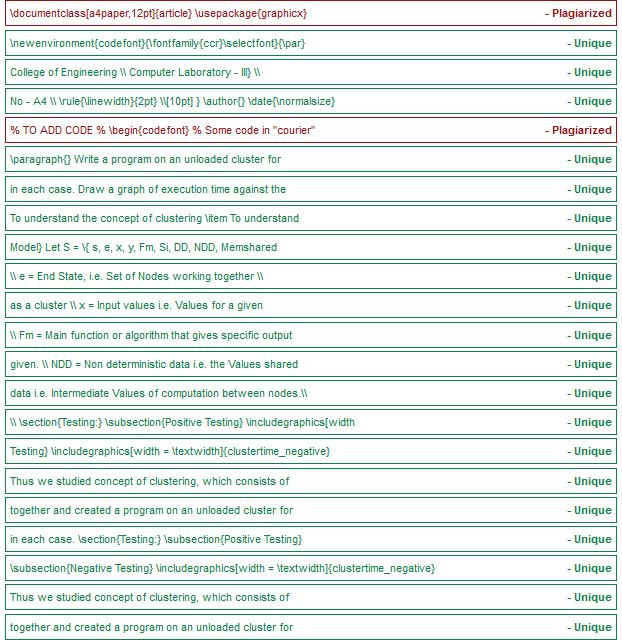
\includegraphics[width=\textwidth]{clustertime_plaga}
\end{document}
 

 
